\section{Fuzzy Clustering}
\label{sec:fuzzy}

%(metastable decomposition induced by zeros of eigenfunctions)?
The above considerations result in a metastable full decomposition of the state space, assigning each state to \textbf{exactly} one of the partition sets.
%taking into consideration
%Now we show that
In fact, there exist better solutions, considering the fact that states in transition regions are adjacent to several conformations and therefore cannot be uniquely assigned to one of them.
%can belong to several metastable conformations.
We introduce a more general method, allowing some ``overlap'' of the conformations.
%metastable sets/conformations
%in the assignment of states to conformations.
%wer hat diese Methode introduced?? see...
%there may be some overlap in the assignment of states to metastable sets.

% a transition region can be %assigned to several macro states with different weight/degree/probability

\subsubsection*{Set-based vs. Function-based Approach}
The intuitive approach to decompose the state space of a process is to determine a certain number of metastable sets which form a full partition, such that each state belongs to exactly one of the metastable sets.
%is assigned, belongs
%each partition corresponds to one conformation/ metastable set.
The problem with that approach is that likewise each state in a transition region has to be assigned to one of these partition sets. Though why would you assign a state in a transition region to one particular adjacent metastable set and not to another one? Such a strict assignment is obviously not an accurate description of the actual behaviour of the process.
%rigorous,precise,accurate

Therefore this \textit{set-based} clustering method has been replaced by a \textit{function-based} method.
That means that the states of the process are assigned with certain ``degrees'' to the conformations.
This approach is justified by the existence of transition regions.
A state inside of a transition region (around local energy maximum) can enter into different adjacent conformations with similar probabilities.
Therefore, instead of assigning it to a single conformation, we define that it should belong to each of these adjacent conformations with a certain degree.
% and thus, can be interpreted to belong to these conformations with a certain degree.
%maybe it cannot be uniquely assigned to a single conformation.
In that sense, the conformations may be ``overlapping''.


\subsubsection*{Membership Functions}

%reversible
Assume we are given a transfer operator having $n$ dominant eigenvalues. Hence, we want to create a Markov State Model on $n$ states, corresponding to the metastable sets of the process.
We follow the approach of Weber\cite{weber2006meshless} to define macro states as \textit{overlapping partial densities}.
%Each macro state is identified by a membership function $\chi_j$ that assigns to each micro state a degree of membership to belong to this conformation.
They can be identified by membership functions that assign degrees of membership to the micro states.
%signifying

%Each state of the original state space shall be assigned to the different macro states with a certain \textit{degree of membership}.

%So far, we were speaking about partition of unity, but with the fuzzy terminology in mind it makes sense to call them membership functions; as they determine the portion of membership to each conformation
\begin{defi}[Membership Function]
% (see \ref{sec:galerkin})
The functions $\cfam : E \rightarrow [0,1]$ are called \textit{membership functions} if they fulfill
\begin{itemize}
\item $\chi_j(x) \geq 0$ $\forall i \in E$ and $\forall j \in \{1,\dots,n\}$ (positivity),
\item $\sum_{j = 1}^n \chi_j(x) = 1$ $\forall x \in E$ (partition of unity).
\end{itemize}
The value $\chi_j(x)$ is the \textit{degree of membership} of state $x$ to macro state $\chi_j$.
%\marginpar{conf. $j$ or $\chi_j$?}
\end{defi}
%membership fct. = part. of unity? Here: yes. Röblitz: required that each function takes value 1

The example of a full-partition discretization corresponds to the choice of characteristic functions $\{ \eins_{A_1},\dots, \eins_{A_n} \}$ as membership functions. Each micro state is uniquely assigned to one of the partition sets, without any overlap.
Therefore such a clustering is called \textit{crisp} or \textit{hard}, whereas the general, possibly overlapping, membership functions result in a \textit{fuzzy} or \textit{soft} clustering.
As there are many possible membership functions, we need to find a choice that yields a reasonable metastable decomposition.
%Usually they look like that

%It turns out that a good choice are membership functions that are
Usually they are chosen to be \textbf{close} to a characteristic function, also called \textit{almost characteristic function}, as depicted in \ref{fig:fuzzy}.
%region,conformation. reasonable/makes sense
%This choice makes sense,
This is a reasonable choice, since it puts the emphasis of a conformation on a certain region by assigning a high degree of membership,
%and maybe some adjacent parts (low degree of membership), but also takes into consideration the critical behaviour of transition regions.
though likewise includes the adjacent transition regions by a low degree of membership.
Thus, they fulfill the following two desired conditions:
\begin{itemize}
\item There should be a \textbf{soft} assignment inside of a transition region, in order to respect the ambiguous membership of transition states.
%Transition regions should be handled carefully, i.e. there should be a \textbf{soft} assignment,
\item The clustering should be \textbf{crisp} enough to distinguish the conformations.
%Different conformations should be clearly visible, so the clustering should be \textbf{crisp} enough to distinguish the conformations.
\end{itemize}

\begin{figure}[!ht]
	\centering
	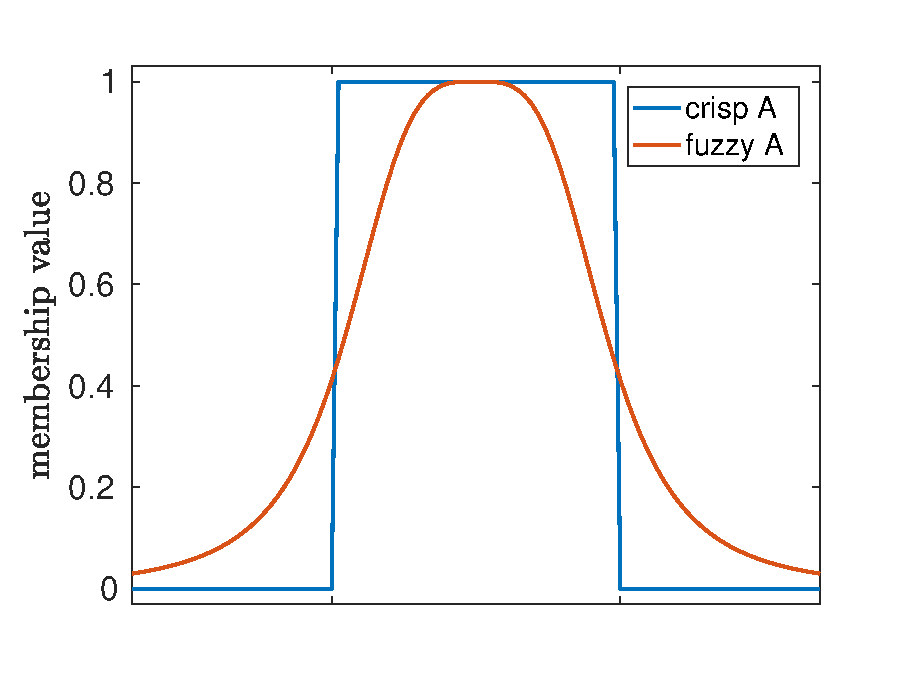
\includegraphics[width=0.4\textwidth]{figures/fuzzy/fuzzy3.eps}
 	\caption{The crisp set $A$ represented by a characteristic function is approximated by a fuzzy set represented by an ``almost characteristic function''.}
        \label{fig:fuzzy}
\end{figure}

These requirements are clarified in figure \ref{fig:membership} at the recurring example of a double-well potential, i.e. a system consisting of two conformations with one transition region between them. A crisp clustering does not consider the transition region, while a ``very fuzzy'' choice of membership functions does not represent the conformations.

\begin{figure}
	\centering
	\subfigure[Characteristic functions resulting in a hard clustering.] {\includegraphics[width=0.4\textwidth]{figures/fuzzy/indicator2.eps}}
	\subfigure[Almost characteristic functions resulting in a soft clustering.]{\includegraphics[width=0.4\textwidth]{figures/fuzzy/almost2.eps}}
%	\includegraphics[width=0.3\textwidth]{figures/fuzzy}
	\caption{Possible membership functions: From hard to fuzzy clustering.}
	\label{fig:membership}
\end{figure}

%Conceptually, they are no probabilities
The degrees of membership are no actual probabilities, yet they can be interpreted as such.
%In the case of a full-partition discretization, the probability of a micro state to belong to a certain conformation is $1$, while the probability to be in any other conformation is $0$, which is obvious by the unique assignment of micro states to the conformations.
Consider for instance the energy maximum of a symmetric double well potential. This transition state tends with the same probability to the left and to the right well. Therefore it seems plausible to assign it with the same degree of membership to both conformations.
On the other hand, a state in the middle of a well cannot immediately jump into the other well, therefore this transition probability is $0$ and the state can be assigned with degree of membership $1$ to the conformation corresponding to its well.
\\

%improvement/enhancement. fuzzyness/overlap
%In figure \ref{fig:membership}, we can clearly see the advantage of using almost characteristic functions as membership functions. Since they allow a soft assignment of the transition region, they are an improvement in comparison to characteristic functions.
%Nevertheless, the functions should not be ``too fuzzy'', since otherwise the disctinction between the conformations can be blurred. Thus some overlap is good, but we also need a certain crispness, in order to identify different conformations.
%identify,distinguish

%another way to explain the meaning of membership functions; interpretation as partial densities
For each conformation $j \in \{ 1 , \dots, n \}$, there is a membership function $\chi_j$ which determines the portion of the partial density with respect to the total density function. \marginpar{?}
They form a partition of unity, in order to sum up to the total density.
%Sometimes the $\chi_j$ will also be called conformation.
In the following, the $\chi_j$ will also be denoted as the conformation $j$ they represent.
%some density function given? t.ex. Boltzmann distribution
%Weber Diss 10
\\

In order to represent the conformations as almost invariant sets, almost characteristic functions should be almost eigenfunctions of the transfer operator:
%having invariant sets
%As characteristic functions are right eigenvectors of a uncoupled(!) transition matrix, the following should be true for almost characteristic functions, thus for membership functions: \marginpar{??}
%perturbation analysis
\begin{equation*}
\Pcal \chi_j \approx \chi_j \ \forall j=1,\dots,n.
\end{equation*}
%\begin{equation*}
%\Qcal \chi_j \approx 0 \ \forall j=1,\dots,n.
%\end{equation*}
%\begin{equation*}
%P_c \chi_j \approx \chi_j \ \forall j=1,\dots,n.
%\end{equation*}
%\begin{equation*}
%T\chi_j \approx S\chi_j \ \forall j=1,\dots,n.
%\end{equation*}
%\pagebreak

%Meaning of the Matrix Representation of the Galerkin Projection
%\subsubsection*{Galerkin Projection} %(Matrix Representation)
\subsubsection*{Matrix Representation of Projection} %(Matrix Representation)

Having determined the shape of the membership functions, we can apply the Galerkin projection as defined in section \ref{sec:galerkin}.
If we choose almost characteristic functions representing the (fuzzy) conformations, then the resulting Markov State Model consists of the metastable sets of the original process.
%represents the metastable sets of the original process
%More precisely, each membership function is an almost characteristic function representing a fuzzy conformation. \marginpar{?}
We remember the matrix representation $P_c = S\inv T$ of a clustered process.
The trace of the coupling matrix $T$ is referred to as \textit{metastability} of the conformations $\{\cfam\}$.
%why that makes sense? high diagonal elements -> high eigenvalues -> high metastability
%Weber meshless p.26

We recall that a full-partition decomposition yields a matrix $S$ being equal to the identity matrix, justified by the orthogonality of the characteristic functions. With the motivation to choose almost characteristic functions as membership functions, the $\chi_i$ are still close to being orthogonal and therefore, $S$ should still be close to the identity matrix, at least diagonal dominant. \marginpar{..}

Thus, we have the coupling matrix $T$, representing the dynamical behaviour of the process.
%Since it should consist of the metastable sets, it should also be a diagonally dominant matrix.
%Now, what is the actual meaning of $S$? Does it ``disturb'' the stochastic matrix $T$ in some sense?
If $S$ is close to the identity matrix, then the dynamics of the projected process is completely determined by $T$. In contrast, if $S$ deviates from identity, then it rather influences the dynamics.

What is the meaning of $S$? The entries are defined by the scalar products of the membership functions.
Thus, the \textit{crispness} of a clustering can be measured by the matrix $S$.
% nonoverlapping = char. fcts.
Nonoverlapping membership functions yield an overlap matrix $S$ equal to the unit matrix.
Overlapping membership functions result in a matrix with non-zero outer diagonal elements.
The higher the outer diagonal elements, the higher the overlap.
Therefore the diagonal of $S$ can be seen as a ``measure of crispness'' of the $\chi_1,\dots,\chi_n$. % conformations/membership functions
%Individual eigenfunctions $\Xcal$ do not overlap since they are orthogonal. But the membership functions %$\chi_j$ as linear combinations of the dominant eigenfunctions might have an overlap.
\\

%\subsubsection*{Statistical Weights} %\marginpar{what for?}

%For each macro state we can assign a statistical weight
Each macro state yields a statistical weight
\begin{equation*}
w_j = \langle \chi_j, \eins \rangle_\mu = \int_E \chi_j(x) \mu(\diff x),
\end{equation*}
describing the ``portion'' of a membership function to the total density function. \marginpar{?}
We remark that the statistical weight vector $w = (w_1, \dots, w_n)$ coincides with the left eigenvector of the matrix representation $P_c$ of the clustered process, see theorem \ref{thm:lefteigenvector}.
%stationary vector/left eigenvector of the clustered process
The diagonal matrix $D = \mathrm{diag}(w_1,\dots,w_n)$ consists of the statistical weights of the membership functions. Then $S = D\inv \langle \chi, \chi \rangle_\mu$ and $T=D\inv \langle \chi, \Pcal \chi \rangle_\mu$, compare theorem \ref{thm:galerkin}. %\marginpar{$TS\inv$ vs $S\inv T$}


\subsubsection*{Perron Cluster Analysis} %\marginpar{finite/cont. vec./fct.}

The term \textit{Perron Cluster Analysis} denotes the objective of clustering a Markov process into metastable sets using the \textit{Perron eigenvalues} respective \textit{Perron eigenfunctions}, being eigenvalues close to $1$ and the corresponding eigenfunctions. %means/denotes
Perron Cluster Analysis respectively its algorithmic implementation PCCA (``Perron Cluster Cluster Analysis'') has been developed by Deuflhard et al\cite{deuflhard2000identification}, employing the sign structure of the dominant eigenvalues of the transition matrix. %\marginpar{set-based approach?}
%as what?
%That approach
This has been improved by Deuflhard and Weber\cite{deuflhard2005robust}
%\marginpar{oder Weber und Galliat?}
%soft/fuzzy
who transformed the system of eigenvectors into a system of membership functions resulting in a fuzzy clustering of the state space of the original process; their algorithm is called PCCA+
(``Robust Perron Cluster Analysis'').
%adapted
Originally, PCCA+ was formulated only for discrete Markov chains, but Weber\cite{weber2011subspace} extended it even on continuous processes.
%we present here the more general case for cont. processes with a given transfer operator
\\

%Let $\Xcal$ be the eigenvector matrix, \marginpar{eigenfct.?} i.e. the $i$-th column of $\Xcal$ is an %eigenvector corresponding to the eigenvalue $\lambda_i$. \marginpar{only dom. spec.}

Let $\Pcal := \Pcal(\tau)$ on $L^2(\mu)$ be the transfer operator describing a \textbf{reversible} process, that is $\Pcal$ is $\mu$-self-adjoint, see theorem \ref{thm:selfadjoint_reversible}.
We consider the set of dominant eigenvalues $\{\lfam\}$ with the corresponding set of eigenfunctions $\Xcal = \{\xfam\}$.
They fulfill the eigenvalue problem $\Pcal \Xcal = \Xcal \Lambda$ of the transfer operator $\Pcal$, where $\Lambda = \mathrm{diag}(\lfam)$.
The set of membership functions $\chi= \{\cfam \}$ can be built as a linear combination $\Xcal \Acal$ of the dominant eigenfunctions, that is
\begin{equation}
\label{eq:pcca}
\chi_j(x) = \sum_{i=1}^n \Acal_{ij} \Xcal_i(x), \ j=1,\dots,n.
\end{equation}
%properties/constraints
Here,  $\Acal = \{\Acal_{ij}\}_{i,j=1,\dots,n} \in \R^{n\times n}$ is a real matrix which has to be chosen in such a way that the resulting membership functions $\chi$ fulfill the positivity and partition of unity constraints.
%Noe Lecture 4 (MSM 2015) 
As there are infinitely many such transformations $\Acal$ of the eigenfunctions, we have to determine one that satisfies some optimality condition.
%resulting in a soft membership matrix,
%Consequently,
The algorithm PCCA+ computes the transformation matrix $\Acal$ as the solution of a \textbf{convex} maximization problem, see Weber\cite{weber2006meshless}. %\marginpar{optimal metastability?}
%yields
%In order to fulfill the partition of unity property of each $\chi_i$, the matrix $A$ has to be chosen s.t. $\chi$ %is row-stochastic.
With the resulting membership functions, the Galerkin projection is %computed/given by %(see chapter 1)
\begin{equation}
\label{eq:galerkin2}
	P_c(\tau)  = G(\Pcal(\tau)) = (\langle \chi, \chi \rangle_\mu)\inv (\langle \chi, \Pcal(\tau) \chi \rangle_\mu).
\end{equation}

%\marginpar{only conv. lin.comb.}
Weber\cite{weber2011subspace} shows that for any linear combination of the eigenfunctions $\chi = \Xcal \Acal$, the discretization error of the Galerkin projection vanishes. Hence diagram \ref{fig:diagram_transfer} commutes, implying that propagating and projecting of a transfer operator are commutative actions. In particular, such membership functions preserve the Markov property.
%In particular, such a choice of membership functions preserves the Markov property.
%Markovianity
\begin{thm}[Weber {\cite[Theorem 2]{weber2011subspace}}]
	\label{thm:iteration_error}
	Let $\Pcal := \Pcal(\tau)$ be a $\mu$-self-adjoint transfer operator with a set $\Xcal = \{ \Xcal_1,\dots, \Xcal_n\}$ of normalized eigenfunctions s.t. $\Pcal \Xcal = \Xcal \Lambda$, where $\Lambda = \mathrm{diag}(\lambda_1,\dots,\lambda_n)$ is the eigenvalue matrix.
	Let $\chi = \Xcal A$ be a set of functions that is a linear combination of the eigenfunctions $\Xcal$ with a regular $n \times n$-transformation matrix $A$ as defined in \eqref{eq:pcca}.
	Then the iteration error for the Galerkin discretization $P_c = G(\Pcal)$ vanishes. %in \eqref{eq:galerkin2}
\end{thm}
\begin{proof}
	%weber p.32
	%We compute the Galerkin projection on the transfer operator $\Pcal$:
	The Galerkin projection of the transfer operator $\Pcal$ is computed by
	\begin{align*}
	G(\Pcal) \; & \stackrel{\mathclap{\eqref{eq:galerkin2}}}{=}  \;
	(\langle \chi, \chi \rangle_\mu)\inv (\langle \chi, \Pcal \chi \rangle_\mu) \\
	& \stackrel{\mathclap{\eqref{eq:pcca}}}{=} \;
	( A^T \langle \Xcal, \Xcal \rangle_\mu A)\inv ( A^T \langle \Xcal, \Pcal \Xcal \rangle_\mu A) \\
	& = \; ( A^T \langle \Xcal, \Xcal \rangle_\mu A)\inv ( A^T \langle \Xcal, \Xcal \rangle_\mu \Lambda A) \\
	& = \; ( A^T A)\inv ( A^T \Lambda A) \\
	& = \; A\inv \Lambda A.
	\end{align*}
	In particular, after $k$ time-steps we get
	\begin{equation*}
		(G(\Pcal))^k = (A\inv \Lambda A)^k = A\inv \Lambda^k A = G(\Pcal^k).
	\end{equation*}
	%Besides
	%\marginpar{semigroup prop.?}
	The last two lines are obtained by inserting the eigenvalue problem $\Pcal \Xcal =\Xcal \Lambda$ and employing the $\mu$-orthogonality of the eigenfunctions, by theorem \ref{thm:spectrum_operator}, and therefore $ \langle \Xcal, \Xcal \rangle_\mu = \Ical$, being the identity operator. \marginpar{orthogonal by symmetrization trick?}
	%The proof is based on the assumption that the Perron eigenfunctions of $\Pcal$ are orthogonal.
\end{proof}

In this proof, it is essential that the process is reversible. If the process is non-reversible, then the transfer operator is not self-adjoint and possibly possesses complex eigenvalues, leading to complex-valued eigenfunctions, which can not be transformed into meaningful membership functions. %spanning invariant subspace of P
%then the orthogonality of the dominant eigenfunctions is not given anymore. \marginpar{not real}
Thus, in order to tackle non-reversible processes as well, an enhanced method is presented in section \ref{sec:nonreversible}.
%it is necessary to introduce a different concept (section \ref{sec:nonreversible}).
\\

%Nielsen p.37!!!!!

%since computation of eigenfunctions is not easy
Even though the algorithm of PCCA+ is valid for continuous processes defined by a transfer operator $\Pcal$, for real applications a discretization of $\Pcal$ to a matrix $P$ is necessary:
\begin{equation*}
	\Pcal \rightarrow P \rightarrow P_c.
\end{equation*}
% of the state space $E$
One approach for that are direct sampling methods, counting transitions between subsets. However, since long-time simulations are required in order to obtain valuable informations about transition between metastable sets, they are not the best choice. Another option are adaptive sampling methods, for instance Voronoi tesselation, see Weber\cite{weber2011subspace}. \marginpar{?}
Having a discrete matrix $P$, it is easy to compute the eigenvalues and eigenvectors in order to apply PCCA+ to get a clustered matrix $P_c$.
In this thesis, we circumvent this first discretization step, by directly examining finite matrices $P$. %are not confrontated

%If we project a finite process, then the above formulation yields a \textit{membership vector matrix} $\chi$, which is the result of a linear combination of the \textit{eigenvector matrix}.
%\newpage

\subsubsection*{Objective Function: Crispness of Membership Functions}
%Weber Diss 58

%Moreover, 
The matrices $S$ and $T$ from the matrix representation $P_c$ can be expressed as
\begin{equation}
\label{eq:projection_presentation2}
\begin{aligned}
T & = D^{-1} \langle \chi, \Pcal \chi \rangle_\mu = D^{-1}A^T \Lambda A \ \ \textrm{ and } \\
S & = D^{-1} \langle \chi, \chi \rangle_\mu = D^{-1} A^T A.
\end{aligned}
\end{equation}

Different objective functions are possible, some are proposed in Weber\cite[Chapter 3.4]{weber2006meshless}.
Originally, one objective was to maximize metastability by maximizing $\mathrm{trace}(T)$.
In the context of stochastic matrices, a high trace of corresponds to a high determinant, since $\trace(T)$ is bounded by above from $n$ and $\det(T)$ by $1$.
This upper bound is achieved only for the case of the identity matrix, thus for a ``strong diagonal''.
Trying to increase the trace to being close to $n$ is the same as increasing the determinant to being close to $1$.
Since the trace is not multiplicative, we resort to the determinant to calculate the following relation:
\begin{align*}
\det(T) & = \det(S) \det(A\inv \Lambda A)  \\
		  & = \det(S) \det(\Lambda)			 \\
          & = \det(S) \Pi_{i=1}^n \lambda_i.
\end{align*}
In order to obtain a high metastability of the system, both factors need to be high.
%In order to increase the metastability of a system, both factors need to be high.
%determinants need to be high.
The term $\det(\Lambda)$ is high if the dominant eigenvalues $\lambda_i$ are as close as possible to $1$, whereas $\det(S)$ is maximized if the linear combination $\chi = \Xcal \Acal$ is as \textbf{crisp} as possible.
That means that they are as orthogonal as possible, having only few overlap.
Since $S$ is a stochastic matrix as well, maximizing its determinant is equivalent to maximizing its trace.

%makes sense
Thus the choice of maximizing $\trace(S)$ as objective function for PCCA+ is plausible, since it provides a clustering with high metastability, while the metastable sets are well distinguishable because of the crispness.  This was proposed by R\"oblitz\cite{roblitz2009statistical}.
Moreover, $\trace$ is a \textbf{convex} function, which is a necessary criterion for the objective function of PCCA+:
\begin{equation}
\label{eq:crispness}
\max_{A \in \R^{n \times n}} \trace(S) \ \ \textrm{such that} \ \chi = XA \geq 0 \ \mathrm{and} \ \sum_j \chi_{ij} = 1. 
\end{equation}
%\\

%Different objective functions are possible. The intuitive optimization criterion would be to maximize the metastability of the membership vectors such that the resulting clustering is ``optimal'' with respect to metastability. However, a different optimization criterion is to make the membership vectors as ``crisp'' as possible by maximizing the trace of the matrix $S$.
%That means that they should be as orthogonal as possible. This was proposed by R\"oblitz\cite{roblitz2009statistical}.
%Thus the objective function used in PCCA+ is given by
%PCCA+ solves the constrained optimization problem

%The trace of $S$ is at most $n$. Optimizing $\mathrm{trace}(S)$ is equivalent to optimizing the \textit{crispness} of the conformations $\chi$ (Röblitz). -> high metastab.

%Better: linear combination of eigenfunctions (might have an overlap) (membership functions, PCCA+).

\subsubsection*{Example}
\clearpage